\begin{figure*}[p!]
  \centering
  \subfloat[Body frame angle]{
    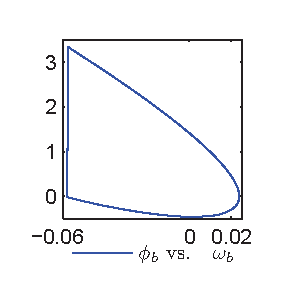
\includegraphics[width=0.24\textwidth]{pp-time-1-s}
    \label{fig:pp-t-ref}
  }
  \subfloat[Ankle angles]{
    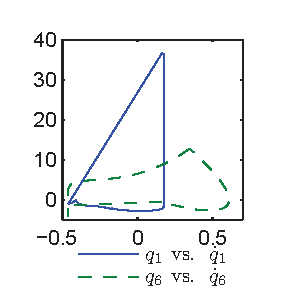
\includegraphics[width=0.24\textwidth]{pp-time-2-s}
    \label{fig:pp-t-ankle}
  }
  \subfloat[Knee angles]{
    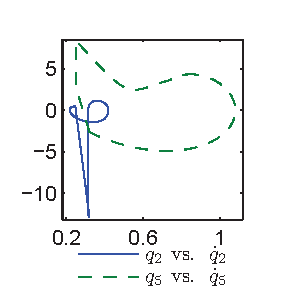
\includegraphics[width=0.24\textwidth]{pp-time-3-s}
    \label{fig:pp-t-knee}
  }
  \subfloat[Hip angles]{
    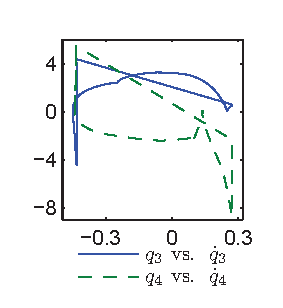
\includegraphics[width=0.24\textwidth]{pp-time-4-s}
    \label{fig:pp-t-hip}
  }
  \caption{Phase portraits of simulation of time-based system $\HS_t$.}
  \label{fig:pp-t}
  \vspace{-7mm}
\end{figure*}

\begin{figure*}[p!]
  \centering
  \subfloat[Body frame angle]{
    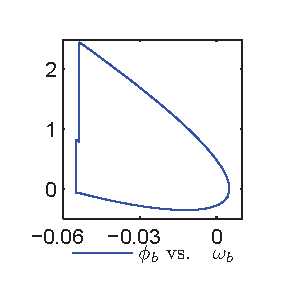
\includegraphics[width=0.24\textwidth]{pp-auto-1-s}
    \label{fig:pp-a-ref}
  }
  \subfloat[Ankle angles]{
    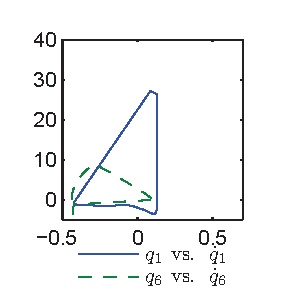
\includegraphics[width=0.24\textwidth]{pp-auto-2-s}
    \label{fig:pp-a-ankles}
  }
  \subfloat[Knee angles]{
    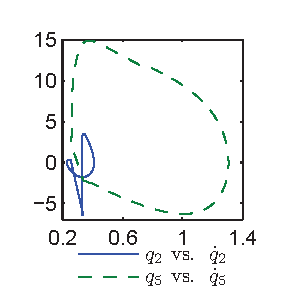
\includegraphics[width=0.24\textwidth]{pp-auto-3-s}
    \label{fig:pp-a-knee}
  }
  \subfloat[Hip angles]{
    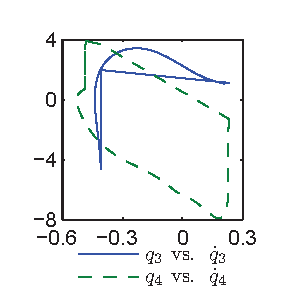
\includegraphics[width=0.24\textwidth]{pp-auto-4-s}
    \label{fig:pp-a-hip}
  }
  \caption{Phase portraits of simulation of autonomous system $\HS_a$.}
  \label{fig:pp-a}
\end{figure*} 
